\documentclass{beamer}
\mode<presentation>{\usetheme{Icy}}

\usepackage{amsmath,amssymb}
\usepackage[english]{babel}
\usepackage[size=custom,width=120,height=75,scale=1]{beamerposter}
\usepackage{booktabs,array}
\usepackage{listings}
\usepackage{xspace}
\usepackage{fp}
\usepackage{ifthen}
\usepackage{multirow}

\listfiles
\newcommand*{\signstream}{SignStream\texttrademark\xspace}

\title{\Huge Dispersion Estimation and Its Effect on Test Performance in RNA-seq Data Analysis}

\author{Will Landau and Dr. Peng Liu}
\institute[Iowa State University]
{Iowa State University, Ames, IA, USA}
\date[August 5, 2013]{August 15, 2013}

\begin{document}
\begin{frame} 
\begin{columns}[t]

\begin{column}{.33\linewidth}


\begin{block}{Abstract}
\setkeys{Gin}{width=.45\textwidth}
\begin{flushleft}
\hspace{1cm} A central goal of RNA sequencing (RNA-seq) experiments is to detect differentially expressed genes. In the ubiquitous negative binomial model for RNA-seq data, each gene is given a dispersion parameter, and correctly estimating these dispersion parameters is vital to detecting differential expression. Since the dispersions help control the variances of the gene counts, underestimation may lead to false discovery, while overestimation may lower the rate of true detection. The simulation study here compares several existing dispersion estimation methods in terms of point estimation and performance in tests for differential expression. The methods that maximize the test performance are the ones that use a moderate degree of dispersion shrinkage: the DSS, Tagwise wqCML, and Tagwise APL methods. In practical RNA-seq data analysis, we recommend using one of these moderate-shrinkage methods with the QLShrink test in {\tt QuasiSeq} R package.
\end{flushleft}
\end{block}


    
\begin{block}{Modeling RNA-seq data}

\begin{itemize}
\item Negative Binomial (NB) model for the expression level of gene $g$ in sample $i$:
\begin{align*}
y_{g, i} &\sim \text{NB(mean = } \mu_{g, i}, \ \text{dispersion} = \phi_g)  \\
\mu_{g, i} &= s_i \cdot \nu_{g, k(i)} \\
k(i) &= \text{Treatment group of sample $i$} \\
s_i &= \text{Normalization factor of sample $i$} 
\end{align*}
\item Dispersion $\phi_g$ controls the variance.
\begin{align*}
Var(y_{g,i}) &= \mu_{g, i} + \mu_{g, i}^2 \cdot \phi_g 
\end{align*}
\item Overestimating dispersions may lead to false negatives, while underestimating dispersions may lead to false positives.
\end{itemize}
\end{block}
    
\begin{block}{Existing methods for estimating dispersions}
\begin{center}
\begin{tabular}{lll}
{\bf Method} $\qquad$ & {\bf Description} & {\bf Authors} \\ \hline
QL & Quasi-Likelihood & cited by Robinson and Smyth (2008) \\ \hline
DSS & Dispersion Shrinkage for Sequencing & Wu, Wang, and Wu (2012) \\ \hline
wqCML & Weighted Quantile-Adjusted  & Robinson and Smyth (2008) \\ 
& Conditional Maximum Likelihood & \\ \hline
APL & Cox-Reid Adjusted Profile Likelihood $\qquad $& McCarthy, Chen, and Smyth (2012) \\ \hline
DESeq & Differential Expression for Sequence  & Anders and Huber (2010) \\
& Count Data &
\end{tabular} 
\end{center}
\end{block}

\begin{block}{Most methods shrink dispersions towards a common value, trend, or prior distribution.}
\begin{center}
\begin{tabular}{ll}
{\bf Method }$\qquad$& {\bf Dispersion shrinkage options } \\ \hline
QL & None \\ \hline
DSS & Empirical Bayes model with a shared log-normal prior for the $\phi_g$'s. \\ \hline
wqCML & Common: maximize shared log likelihood, $l_S(\phi_g)$  \\
& Tagwise: maximize weighted log likelihood, $l_g(\phi_g) + \alpha \cdot l_S(\phi_g) $\\ \hline
APL & Common: maximize $APL_S(\phi_g) = \frac{1}{G} \sum_{g' = 1}^G APL_{g'}(\phi_g)$ \\
& Trended: Restrict $\phi_g$'s to a trend and maximize $APL_g(\phi_g)$. \\
& Tagwise: Use local mean APL ($APL_{S_g}$) and maximize $APL_g(\phi_g) + \alpha \cdot APL_{S_g}(\phi_g)$  \\ \hline
DESeq & None  \\
& Trended: fit $\phi_g$'s to trend. \\
& Maximum: take $\phi_g$ to be the maximum of the raw estimate and trend. 
\end{tabular}
\end{center}
\end{block}
    
    

\end{column}    











%%%%%%%%%%%
\begin{column}{.33\linewidth}



\begin{block}{The simulation study}
\begin{itemize}
\item 30 datasets (2 treatment groups and 10,000 genes each) were simulated from the negative binomial model under each of the following settings: \newline

\begin{center}
\begin{tabular}{llcc}
Setting & Dataset & Group 1 samples & Group 2 samples \\ \hline
I & Pickrell & 3 & 3 \\ \hline
II & Pickrell & 3 & 15 \\ \hline
III & Pickrell & 9 & 9 \\ \hline
IV & Hammer & 3 & 3 \\ \hline
V & Hammer & 3 & 16 \\ \hline
VI & Hammer & 9 & 9 \\
\end{tabular} 
\end{center} \vspace{1.03cm}

\item In the simulated datasets, the true overall per-gene expression levels and true dispersions were taken from real datasets: \newline

\begin{center}
\begin{tabular}{ccc}
Pickrell: & GSE19480 & human \\ 
Hammer: & GSE20895 & mouse 
\end{tabular}
\end{center}

%\item The true dispersions were compared to the dispersions estimated from the simulated data in terms of:

%\begin{enumerate}
%\item point estimation.
%\item performance when used in five tests for differential expression: 
%\begin{itemize}
%\item The negative binomial exact tests in the {\tt \scriptsize edgeR} and {\tt \scriptsize DESeq} R packages.
%\item QL, QLShrink, and QLSpline: the three quasi-likelihood ratio tests in the {\tt \scriptsize QuasiSeq} R package.
%\end{itemize}
%\end{enumerate}


\end{itemize}
\end{block}




 \begin{block}{Estimation error: simulation setting VI}
\setkeys{Gin}{height=.907\textwidth}
\begin{center}
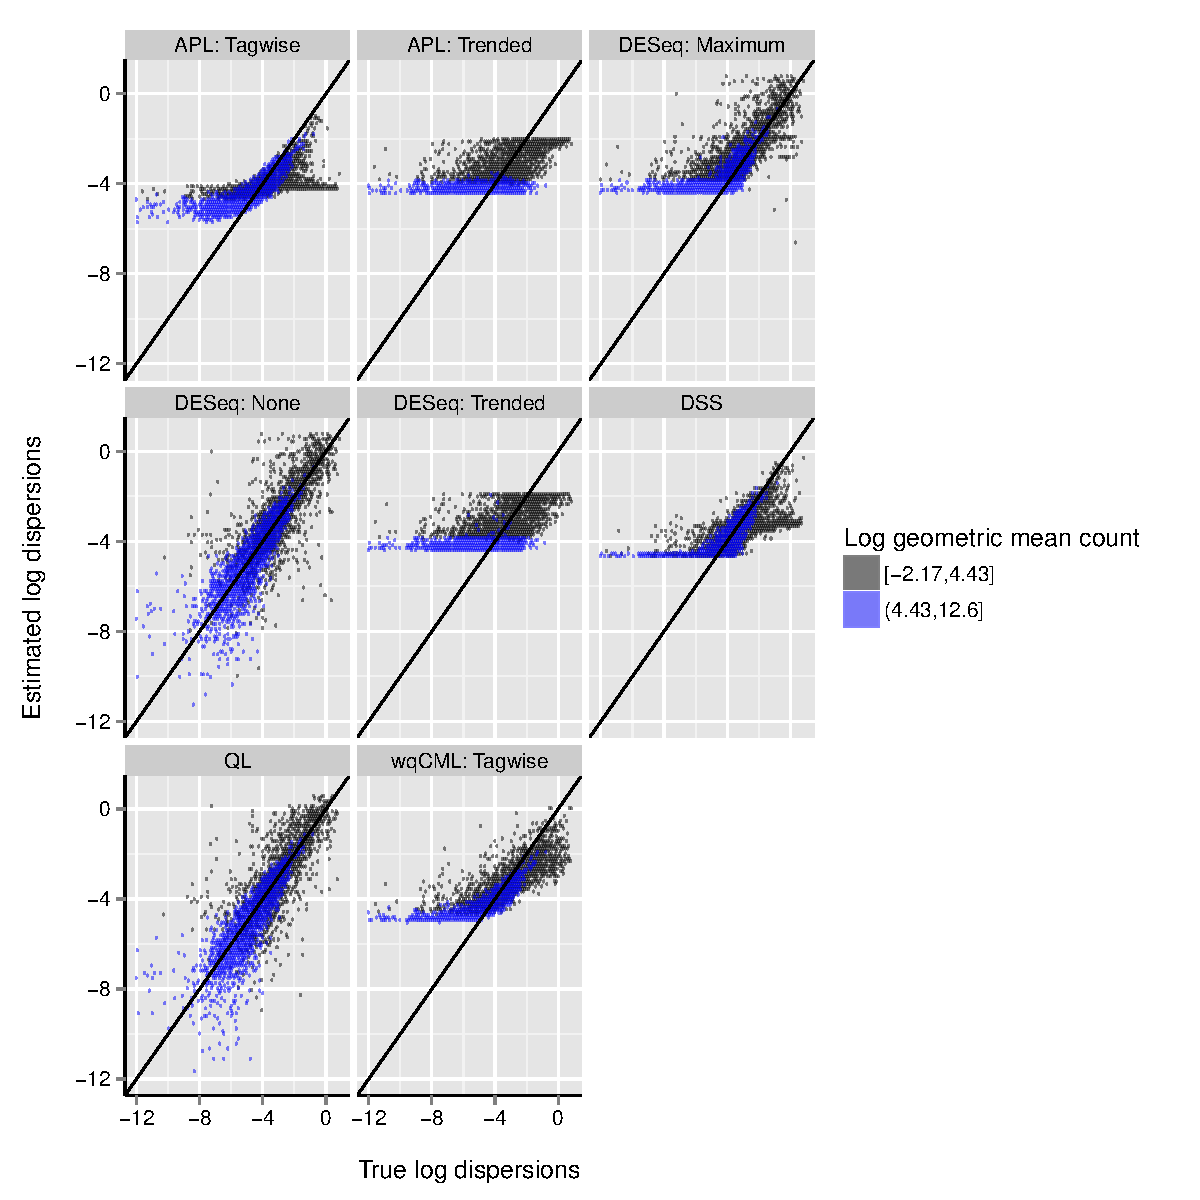
\includegraphics{../fig/phi_vs_phi_VI_slides.pdf} 
\end{center}
\end{block}












\end{column}
\begin{column}{.33\linewidth}





\begin{block}{Mean squared error: simulation settings I through VI}
\setkeys{Gin}{height=1\textwidth}
\begin{center}

\begin{minipage}[l]{0.49\linewidth} \centering
Use the transformed dispersions \\
for calculating mean squared error: \\ 
\begin{align*}
\text{MSE} =  \sum_{g = 1}^G \left (\frac{\widehat{\phi}_g}{1 + \widehat{\phi}_g} - \frac{\phi_g}{1 + \phi_g} \right )^2
\end{align*}
\end{minipage}
\begin{minipage}[r]{0.5\linewidth}
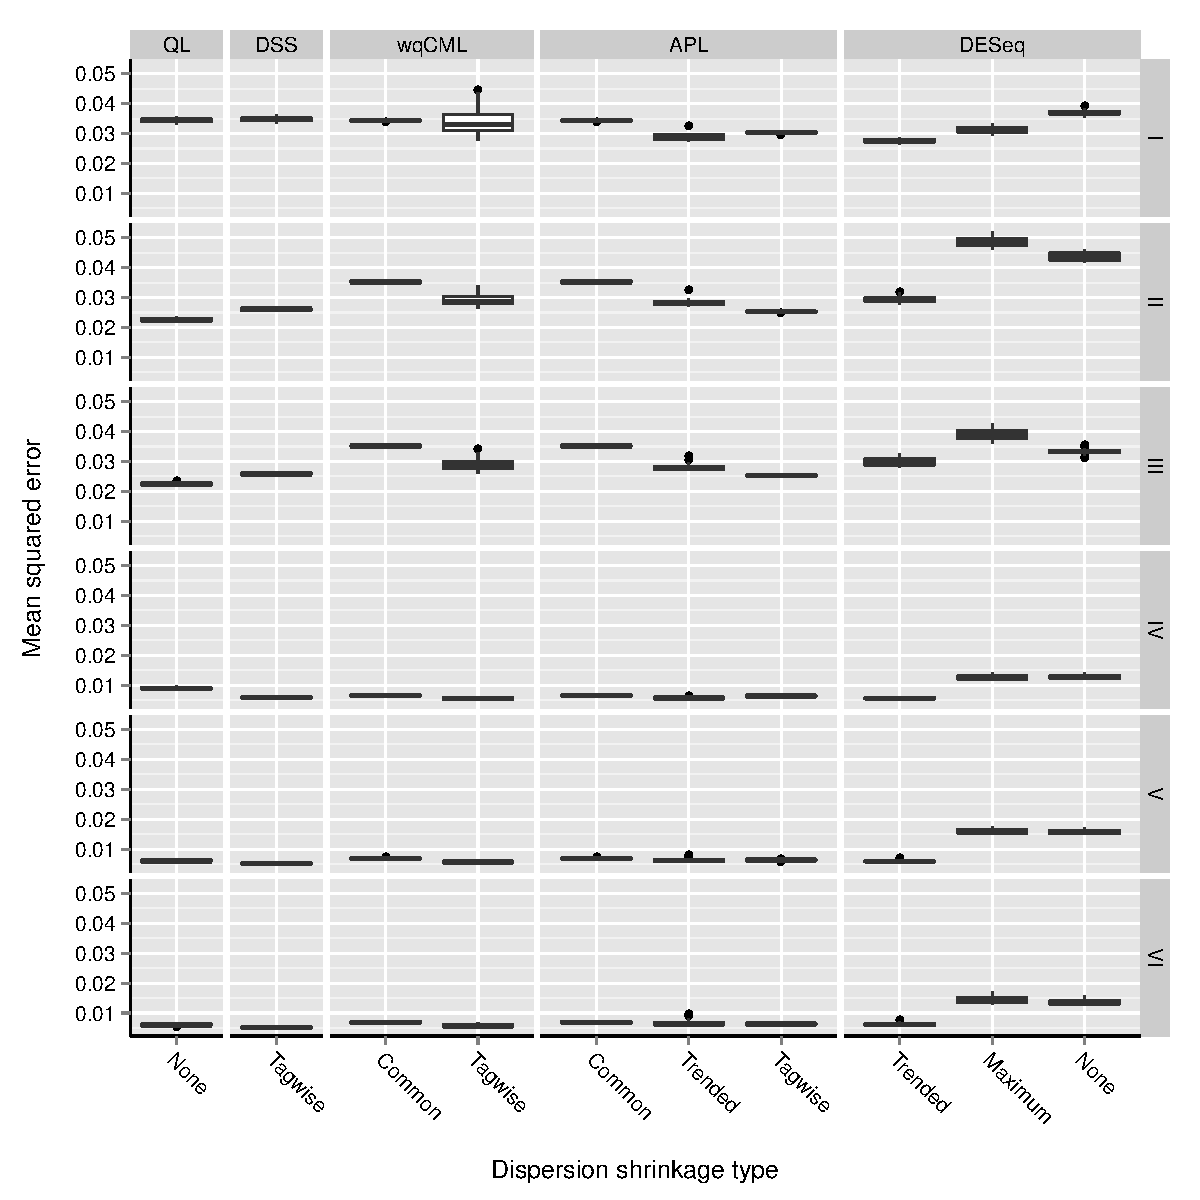
\includegraphics{../fig/mse_slides.pdf}
\end{minipage}

\end{center}
\end{block}

\begin{block}{Performance in five tests for differential expression: simulation settings II (left) and VI (right)}
\setkeys{Gin}{height=.4825\textwidth}
\begin{center}
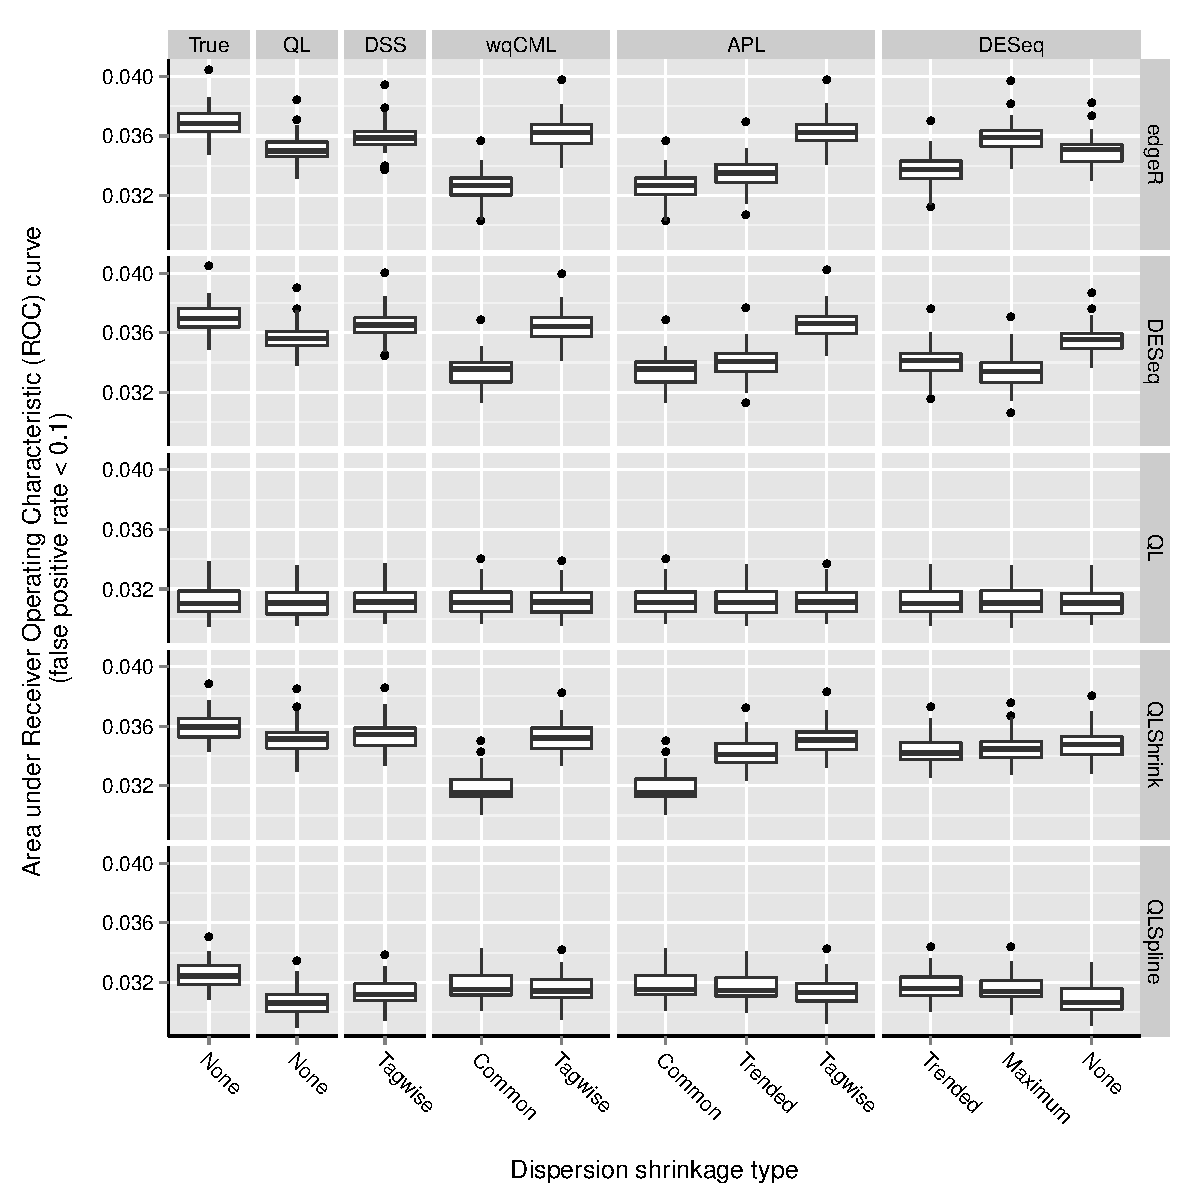
\includegraphics{../fig/auc2_slides.pdf} $\quad$ 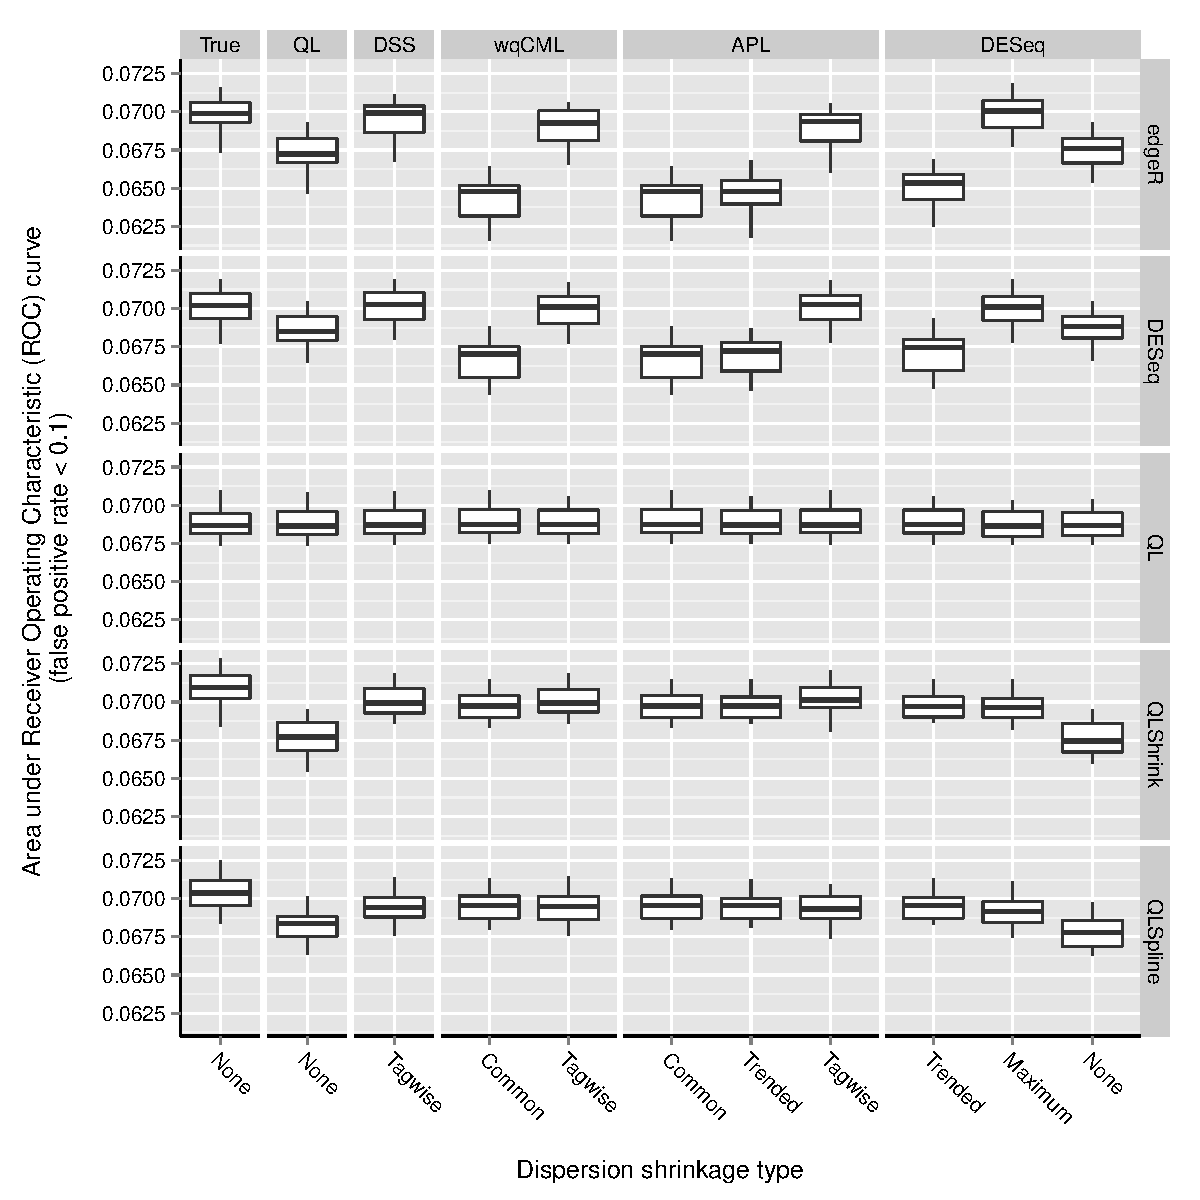
\includegraphics{../fig/auc6_slides.pdf}  
\end{center}
\end{block}




\begin{block}{Conclusions}
\begin{itemize}
\item Best dispersion estimation methods: DSS, Tagwise wqCML, Tagwise APL
\item Best tests for differential expression:
\begin{itemize}
\item edgeR exact test (performance varies with dispersion estimation method).
\item DESeq exact test (performance varies with dispersion estimation method).
\item QLShrink test (more robust robust under dispersion estimation method and departures from the negative binomial model).
\end{itemize}

\item The best dispersion estimation methods use a moderate degree of dispersion shrinkage. However, the \emph{kind} of shrinkage varies within this optimal group.
\item Estimation error is not always indicative of test performance. 
\begin{itemize}
\item Maximum DESeq is one of the worst in terms of mean squared error, but often performs well in tests for differential expression.
\end{itemize}

\end{itemize}
\end{block}    
    


\end{column}

\end{columns}
\end{frame}
\end{document}